\begin{document}
The CMOS ring oscillator consists of three CMOS inverters connected in series with the
output of the last inverter connected to the input of the first inverter. The ring oscillator will also have a
capacitor at each output connected to ground. The schematic for the CMOS ring oscillator can be seen in Figure \ref{fig:ringoscillatorcmosexp}.

\begin{figure}[H]
	\centering
	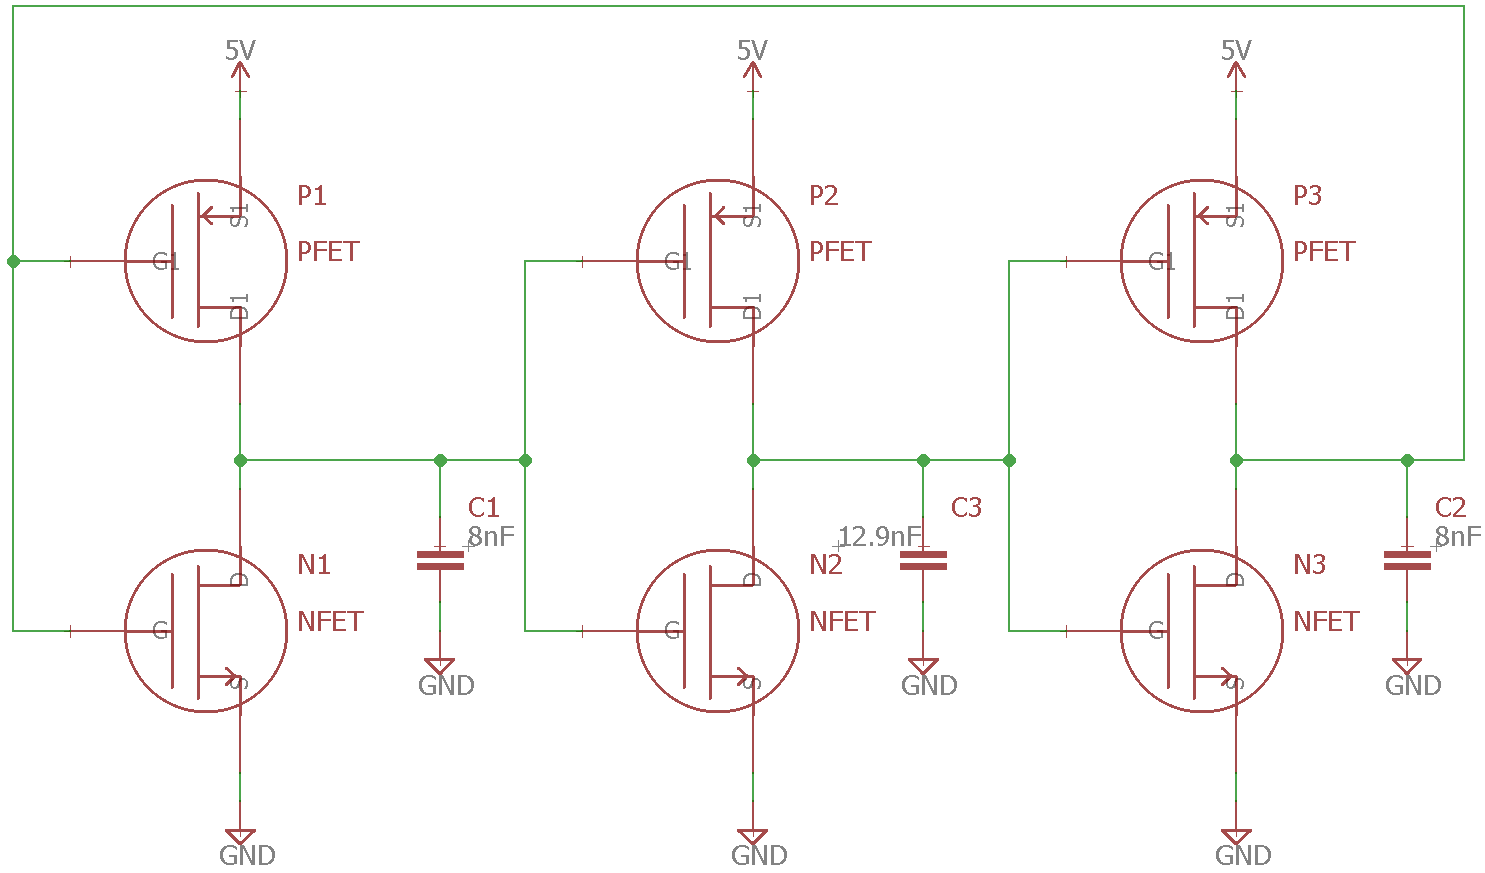
\includegraphics[width=0.5\linewidth]{CircuitDevelopment/RingOscillatorCMOSexp.png}
	\caption{CMOS ring oscillator schematic}
	\label{fig:ringoscillatorcmosexp}
\end{figure}


The operation of the ring oscillator uses a series of inverters. The output of one inverter inverts the input signal. Therefore, if there are a series of inverters, then each odd inverter will have the same inverted output as the first. In this instance, there are three stages of inverters used, with the output of the third inverter being fed back into the input of the first inverter. This feedback from the output to the input causes an oscillation. The simulated output of the ring oscillator is depicted in Figure \ref{fig:ringoscsimlab4}.

\begin{figure}[H]
	\centering
	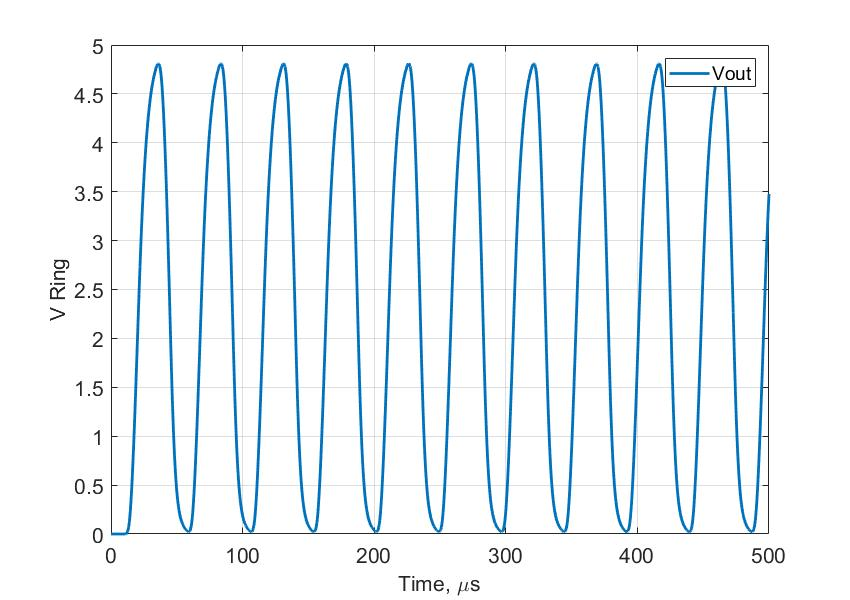
\includegraphics[width=0.6\linewidth]{CircuitDevelopment/ringoscsimlab4.jpg}
	\caption{Simulated CMOS ring oscillator output}
	\label{fig:ringoscsimlab4}
\end{figure}

The output of the ring oscillator seen in Figure \ref{fig:ringoscsimlab4} is not a square wave, but instead a distorted sinusoid. However, the signal will be converted into a square wave by using a schmitt trigger. The resulting signal will be used to drive the LED driver circuit.
 



\end{document}